%% Project Overview goes here
\section{Overview}

This INM460 Computer Vision coursework project consists of creating facial classifiers from supplied image stills and videos of two types: individual and group, labelled and unlabelled respectively as shown in Fig. \ref {fig:data_example}.
\begin{figure}[h]
 \centering 
 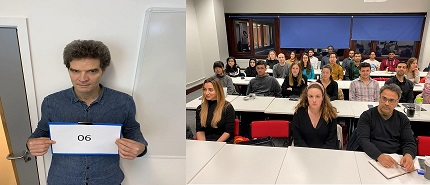
\includegraphics[width=\columnwidth]{images/example-data-50pc.jpg}
 \caption{Example of individual (labelled) and group (unlabelled) images}
 \label{fig:data_example}
\end{figure}

Each individual image contains a sign with a two-digit unique identifier, from which labelled data is obtained to train and test classifier models. 
\subsection{Pre-processing Steps}
For our coursework, the chosen programming language was MATLAB \cite{MATLAB:2018}, version 2018a. All pre-processing steps were sequentially run in script \textbf{ImagePreProcessing.m}, using MATALB user-defined functions:
\begin{enumerate}
\item fnSaveVideoStills
\item fnLabelIndividualImages
\item fnBlurImages
\item fnRotateImages
\item fnCropFaces
\end{enumerate}
In step 1. all videos were saved as stills, with the exception of beginning and ending frames of each video, which were normally black or excessively blurred. In step 2. all images containing unique identifiers which could be recognised through optical character recognition (OCR) with our function \textbf{fnGetStudentID} were moved to a labelled folder, otherwise set aside for manual labelling. Once all images had been identified and moved to labelled folders, totalling 48 labels, we obtained an average of 402 images per label. In steps 3. and 4. the entire data then was augmented by randomly selecting 50\% of each label and applying a random amount of blur to each image, then a further 70\% was randomly selected from each label (including recently added blurred images) and randomly rotated from -10 to 10 degrees.  

The augmented data after step 4. had an average of 1026 images per label. In Step 5. faces were cropped, using MATLAB's vision.CascadeObjectDetector which implements the Viola-Jones algorithm  \cite{990517}, and moved to another set of labelled folders. An average of 985 faces were obtained from each label, which represents approximately 96\% of the augmented data.  
Each label was then manually checked and any images not correctly cropped were removed, resulting in an average of 815 images per label, doubling the size of face image data with respect to stills obtained in step 2. Table \ref {table:preproc} shows label quantities after each processing step, including totals and averages per label.
\begin{table}[h]
\centering
\begin{tabular}{|l|l|l|l|l|l|}
\hline
\multicolumn{6}{|l|}{Pre-processing figures} \\ \hline
Step  &  2 & 3 & 4 & 5 & Final\\ \hline
Total images & 19323 & 28984 & 49273 & 47302 & 39135 \\ \hline
Label avg. & 402 & 604 & 1026 & 985 & 815  \\ \hline
\end{tabular}
\caption{Label quantities after each pre-processing step}
\label{table:preproc}
\end{table}
Fig. \ref {fig:cropped_example} shows examples of three correct face crops, without and with augmentation, and one shoe incorrectly identified as a face.

\begin{figure}[h]
 \centering 
 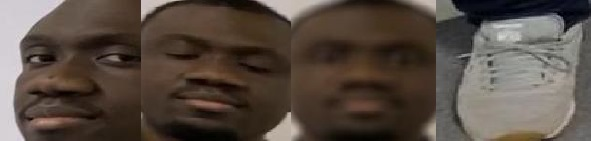
\includegraphics[width=\columnwidth]{images/crop-examples.jpg}
 \caption{Cropped face images including augmented rotated, augmented blurred and misidentified}
 \label{fig:cropped_example}
\end{figure}

\subsection{Determining optimal cropped-face size}

To determine what image size to use for training our models, we examined individual and group images. Files resulting from pre-processing step 5. were square, with varying side dimensions. We used function \textbf{fnStatsCropSizes.m} to calculate the minimum, maximum, median and mode averages of the side of the cropped-face square image (Table \ref{table:face_crop_stats}). 

\begin{table}[h]
\centering
\begin{tabular}{|l|l|l|l|}
\hline
\multicolumn{4}{|l|}{Individual face image side size statistics} \\ \hline
Minimum  &  Maximum & Median & Mode \\ \hline
100 & 252 & 171 & 152 \\ \hline
\end{tabular}
\caption{Rounded average size in pixels for pre-processed images over all labels}
\label{table:face_crop_stats}
\end{table}

We then looked at faces found in group images, both still images, and still images obtained from videos. The latter proved mostly unusable, as the amount of blur did not allow for more than 2 or 3 face images being identified in each frame, so group videos were discarded. We used function \textbf{fnStatsGroupCropSizes.m} to identify face sizes in still group images and obtained cropped face statistics (Table \ref{table:group_crop_stats}).

\begin{table}[h]
\centering
\begin{tabular}{|l|l|l|l|}
\hline
\multicolumn{4}{|l|}{Group face image side size statistics} \\ \hline
Minimum  &  Maximum & Median & Mode \\ \hline
100 & 322 & 128 & 107 \\ \hline
\end{tabular}
\caption{Rounded average size in pixels for pre-processed images over all group images}
\label{table:group_crop_stats}
\end{table}

Since the median side size from faces cropped from group images was 128 and the mode was 107, and group images were the unlabelled data we are looking at classifying, intuitively it seemed to make sense to resize all labelled images closer to the minimum end of the size range, which would require the least amount of resizing to train and test our models, particularly aiming at avoiding to increase the size of cropped faces from group images, introducing some amount of blur. As an example, Figure \ref{fig:decrease_increase_example} shows a sequence where an image of size 217x217 pixels is decreased to size 115x115, with no loss of sharpness, then resized again to 227x227, with some loss of sharpness.

\begin{figure}[ht]
 \centering 
 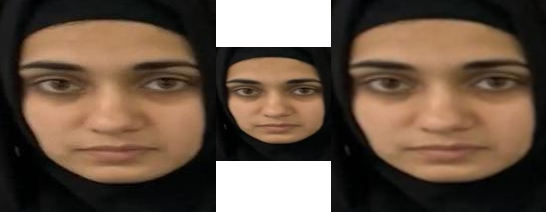
\includegraphics[width=\columnwidth]{images/decrease-increase.png}
 \caption{Sequence showing the effect of decreasing and increasing cropped-face images sizes, from left to right, image is decreased with no apparent loss in sharpness, then increased with some loss in sharpness}
 \label{fig:decrease_increase_example}
\end{figure}

We used function \textbf{fnGetSampleImages.m} to generate sample data for initial models, and based on the results, expanded to full data. We worked with random sets of 50, 100 and 200 images from 8 labels, in three different sizes 227x227, 128x128 and 70x70 pixels, both RGB and grayscale, and then created a few models to test our hypothesis.  

Since a visual inspection showed numerous repetitions in each label, a sample size of 200 images per label was considered sufficient to generate the classifiers.



